\documentclass[11pt, convert={outext=.png}]{standalone}
\usepackage{amsmath}
\usepackage{etoolbox}
\usepackage{ifthen}
\usepackage{tikz}
\usetikzlibrary{math}
\usepgflibrary{patterns.meta}
\usetikzlibrary{patterns.meta}
\usetikzlibrary{shapes.geometric}
\usetikzlibrary{arrows.meta}
\usepgflibrary{arrows.meta}

\makeatletter
\newcommand{\changeoperator}[1]{%
  \csletcs{#1@saved}{#1@}%
  \csdef{#1@}{\changed@operator{#1}}%
}
\newcommand{\changed@operator}[1]{%
  \mathop{%
    \mathchoice{\textstyle\csuse{#1@saved}}
               {\csuse{#1@saved}}
               {\csuse{#1@saved}}
               {\csuse{#1@saved}}%
  }%
}
\makeatother

\changeoperator{sum}

\begin{document}
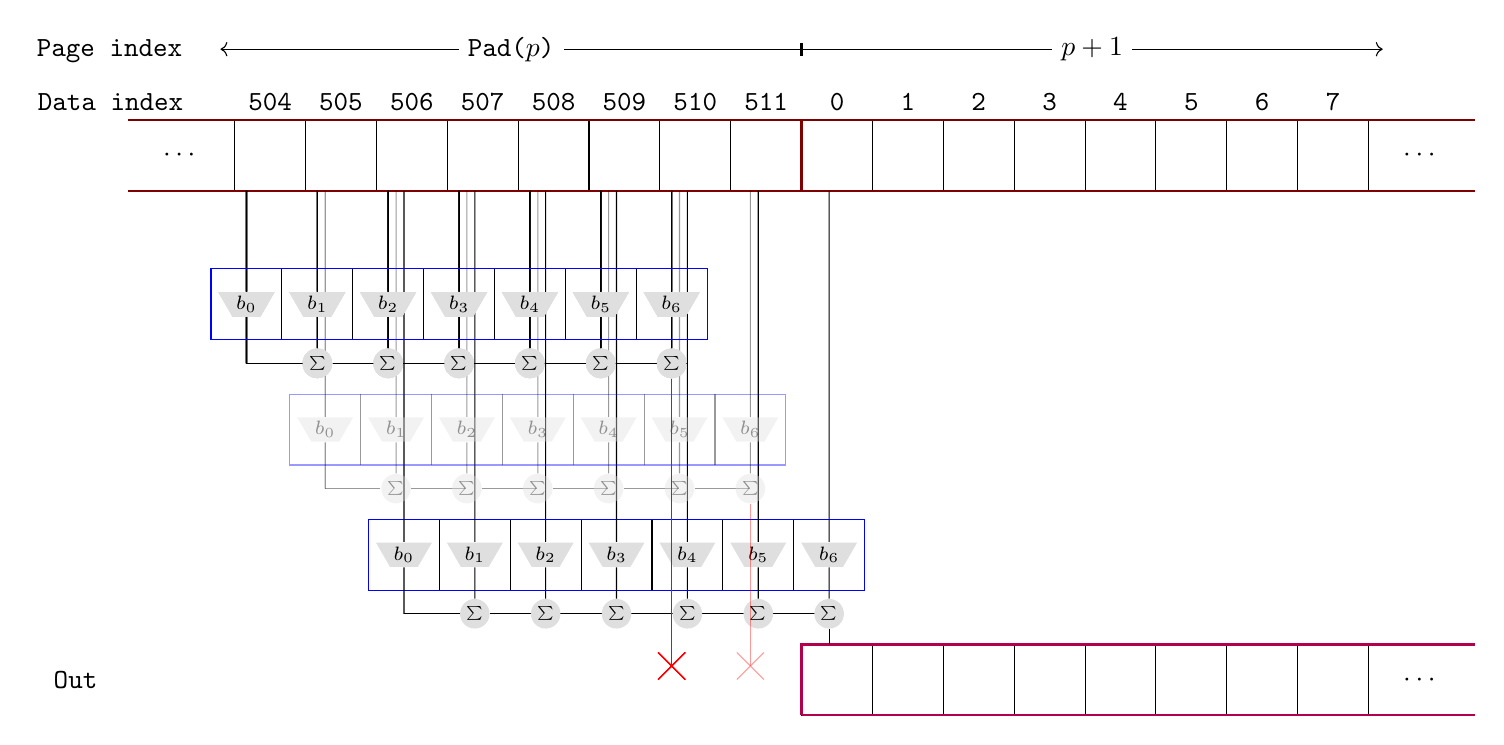
\begin{tikzpicture}
	% Constants
	\tikzmath{
		int \numrect, \totalrect, \dataindex;
		\numrect = 8; \totalrect = int(2 * \numrect);
		\convrectlen = 7; \convrect = int(\convrectlen - 1); \convrows = int(\totalrect - \convrectlen);
		\convrowshide = 2; % This is the number of rows that get rejected
		\convrowsdraw = int(min(\convrows, 3)); % This is the number of convolution rows to draw
		\datawidth = 0.9; \dataheight=0.9; \textstagger=-0.30;
		\rowstagger = 0.1;
		\convstagger = 0.69;
		\outy = \textstagger - (\convrowsdraw + 1) * (\dataheight + \convstagger); % This is the y-coord of bottom of out data
	}

	% In data
	\begin{scope}
		\foreach \i [
			% Each data point
			evaluate=\i as \drawcoord using (\i - \numrect - 1) * \datawidth,
			% Indices associated with point
			evaluate=\i as \nodecoord using (\i - \numrect - 0.5) * \datawidth,
			evaluate=\i as \dataindex using {int(mod(int(\i + 511 - \numrect), 512))},
		] in {1, 2, ...,  \totalrect} {
				% Box for point
				\draw (\drawcoord, 0) rectangle ++(\datawidth, \dataheight);
				% Indices associated with box
				\node[anchor=south] at (\nodecoord, \dataheight) {\texttt{\dataindex}};
			}

		% Page delimiter
		\draw[thick, red!50!black, draw opacity=1.0] ({ -(\numrect + 1.5) * \datawidth }, 0) -- (0, 0) -- (0, \dataheight) -- ({ -(\numrect + 1.5) * \datawidth }, \dataheight);
		\draw[thick, red!50!black, draw opacity=1.0] ({ (\numrect + 1.5) * \datawidth }, 0) -- (0, 0) -- (0, \dataheight) -- ({ (\numrect + 1.5) * \datawidth }, \dataheight);
		% Additional data points
		\node[anchor=center] at ({-(\numrect + 0.75)*\datawidth}, \dataheight/2) {$\cdots$};
		\node[anchor=center] at ({ (\numrect + 0.75)*\datawidth}, \dataheight/2) {$\cdots$};
		% Data index
		\node[anchor=335] at ({-(\numrect + 1.2)*\datawidth}, \dataheight) {\texttt{Data index}};
		% Page index
		\draw[|->] (0, {\dataheight-3*\textstagger}) -- ++({-(\numrect + 0.2)*\datawidth}, 0) node[midway, anchor=center, fill = white] {\texttt{Pad(}$p$\texttt{)}};
		\node[anchor=332] at ({-(\numrect + 1.2)*\datawidth}, {\dataheight-2*\textstagger}) {\texttt{Page index}};
		\draw[|->] (0, {\dataheight-3*\textstagger}) -- ++({ (\numrect + 0.2)*\datawidth}, 0) node[midway, anchor=center, fill = white] {$p+1$};
	\end{scope}

	% Out data
	\begin{scope}
		\node[anchor=east] at ({-(\numrect + 1.8)*\datawidth}, {\outy + \dataheight/2}) {\texttt{Out}};

		% Box for each convolution point. Faked by just drawing divisors
		\foreach \i [ evaluate=\i as \drawcoord using (\i - 1) * \datawidth ] in {1, 2, ...,  \numrect} {
				\draw (\drawcoord, \outy) rectangle ++(\datawidth, \dataheight); % Box for point
			}
		\draw [thick, red!70!blue] (0, \outy) -- ({(\numrect + 1.5)*\datawidth}, \outy);
		\draw [thick, red!70!blue] (0, \outy) -- (0, \outy + \dataheight) -- ({(\numrect + 1.5)*\datawidth}, \outy + \dataheight);
		% Additional data points
		\node[anchor=center] at ({ (\numrect + 0.75)*\datawidth}, \outy + \dataheight/2) {$\cdots$};
	\end{scope}

	% First accepted kernel
	\begin{scope}[opacity=1.]
		\tikzmath {
			\startidx = \convrowshide+1;
		}
		\foreach \rowidx [
			evaluate=\rowidx as \startrectx using (\rowidx - 1 - \numrect) * \datawidth + (\rowidx-int(0.5*\convrows)) * \rowstagger,
			evaluate=\rowidx as \startrecty using \textstagger -(\rowidx - 1 + 1) * \dataheight - (\rowidx * \convstagger),
		] in {\startidx, ..., \convrowsdraw}
			{
				% Box for each convolution point. Faked by just drawing divisors
				\foreach \convidx [
					evaluate=\convidx as \convx using (\convidx * \datawidth + \startrectx),
				] in {1, 2, ..., \convrect}
					{
						\draw(\convx, \startrecty) rectangle ++(0, \dataheight);
					}

				% Total Convolution kernel
				\draw[blue] (\startrectx, \startrecty) rectangle ++(\convrectlen * \datawidth, \dataheight);
				% Conv summation
				\foreach \convidx [
					evaluate=\convidx as \convx using (\convidx * \datawidth + \startrectx),
				] in {0, 1, ..., \convrect} {
						\begin{scope}
							\coordinate (mc) at (\convx + \datawidth/2, \startrecty + \dataheight/2); % Mult center
							\coordinate (sc) at (\convx + \datawidth/2, \startrecty + \textstagger); % Sum center

							\node (mult) [anchor=center, trapezium, trapezium angle=60, fill=gray!25, rotate=180] at (mc) {\phantom {\tiny o}};
							\node[anchor=center] at (mc) {$\scriptstyle b_\convidx$};

							\ifthenelse { \convidx =  0 } {
								\node (sum) [anchor=center, scale=0.0] at (sc) {};
							} {
								\node (sum) [anchor=center, circle, fill=gray!25, scale=0.8] at (sc) {\phantom {\tiny o}};
								\node[anchor=center] at (sc) {$\scriptscriptstyle \sum$}; % amsmath + etoolbox
							}

							\draw (mult.south) -- (mult |-, 0); % Tikz syntax for getting x coord
							\draw (mult.north) -- (sum.north);

							\ifthenelse {\convidx < \convrect}{ \draw (sum.east) -- ++(\datawidth, 0); }
							{ \draw (sum.south) -- (sum |-, {\outy+\dataheight}); } % Draw to right for all but last
						\end{scope}
					}
			}
	\end{scope}

	% Other rejected convolution kernels
	\begin{scope}[opacity=0.4]
		\foreach \rowidx [
			evaluate=\rowidx as \startrectx using (\rowidx - 1 - \numrect) * \datawidth + (\rowidx-int(0.5*\convrows)) * \rowstagger,
			evaluate=\rowidx as \startrecty using \textstagger -(\rowidx - 1 + 1) * \dataheight - (\rowidx * \convstagger),
		] in {2, ..., \convrowshide} {
				% Box for each convolution point. Faked by just drawing divisors
				\foreach \convidx [
					evaluate=\convidx as \convx using (\convidx * \datawidth + \startrectx),
				] in {1, 2, ..., \convrect} {
						\draw(\convx, \startrecty) rectangle ++(0, \dataheight);
					}
				% Total Convolution kernel
				\draw[blue] (\startrectx, \startrecty) rectangle ++(\convrectlen * \datawidth, \dataheight);
				% Conv summation
				\foreach \convidx [
					evaluate=\convidx as \convx using (\convidx * \datawidth + \startrectx),
				] in {0, 1, ..., \convrect} {
						\begin{scope}
							\coordinate (mc) at (\convx + \datawidth/2, \startrecty + \dataheight/2); % Mult center
							\coordinate (sc) at (\convx + \datawidth/2, \startrecty + \textstagger); % Sum center

							\node (mult) [anchor=center, trapezium, trapezium angle=60, fill=gray!25, rotate=180] at (mc) {\phantom {\tiny o}};
							\node[anchor=center] at (mc) {$\scriptstyle b_\convidx$};

							\ifthenelse { \convidx =  0 } {
								\node (sum) [anchor=center, scale=0.0] at (sc) {};
							} {
								\node (sum) [anchor=center, circle, fill=gray!25, scale=0.8] at (sc) {\phantom {\tiny o}};
								\node[anchor=center] at (sc) {$\scriptscriptstyle \sum$}; % amsmath + etoolbox
							}

							\draw (mult.south) -- (mult |-, 0); % Tikz syntax for getting x coord
							\draw (mult.north) -- (sum.north);

							\ifthenelse {\convidx < \convrect}{ \draw (sum.east) -- ++({\datawidth-0.2}, 0); }
							{ \draw [red, arrows = {-Rays[n=4,scale=3]}] (sum.south) -- (sum |-, {\outy+0.5*\dataheight}); } % Draw to right for all but last
						\end{scope}
					}
			}
	\end{scope}

	% First Convolution kernel
	\begin{scope}
		\tikzmath{ % Using the same expression as the scoped block so as to not require manually re-evaluating all coords
			\rowidx = 1;
			\startrectx = (\rowidx - 1 - \numrect) * \datawidth+ (\rowidx-int(0.5*\convrows)) * \rowstagger;
			\startrecty = \textstagger -(\rowidx - 1 + 1) * \dataheight - (\rowidx * \convstagger);
		}
		% Box for each convolution point. Faked by just drawing divisors
		\foreach \convidx [
			evaluate=\convidx as \convx using (\convidx * \datawidth + \startrectx),
		] in {1, 2, ..., \convrect} {
				\draw(\convx, \startrecty) rectangle ++(0, \dataheight);

				\foreach \convidx [
					evaluate=\convidx as \convx using (\convidx * \datawidth + \startrectx),
				] in {0, 1, ..., \convrect} {
						\begin{scope}
							\coordinate (mc) at (\convx + \datawidth/2, \startrecty + \dataheight/2); % Mult center
							\coordinate (sc) at (\convx + \datawidth/2, \startrecty + \textstagger); % Sum center

							\node (mult) [anchor=center, trapezium, trapezium angle=60, fill=gray!25, rotate=180] at (mc) {\phantom {\tiny o}};
							\node[anchor=center] at (mc) {$\scriptstyle b_\convidx$};

							\ifthenelse { \convidx =  0 } {
								\node (sum) [anchor=center, scale=0.0] at (sc) {};
							} {
								\node (sum) [anchor=center, circle, fill=gray!25, scale=0.8] at (sc) {\phantom {\tiny o}};
								\node[anchor=center] at (sc) {$\scriptscriptstyle \sum$}; % amsmath + etoolbox
							}

							\draw (mult.south) -- (mult |-, 0); % Tikz syntax for getting x coord
							\draw (mult.north) -- (sum.north);

							\ifthenelse {\convidx < \convrect}{ \draw (sum.east) -- ++(\datawidth, 0); }
							{ \draw [red, arrows = {-Rays[n=4,scale=3]}] (sum.south) -- (sum |-, {\outy+0.5*\dataheight}); } % Draw to right for all but last
						\end{scope}
					}
			}
		\draw[blue] (\startrectx, \startrecty) rectangle ++(\convrectlen * \datawidth, \dataheight);
	\end{scope}
\end{tikzpicture}
\end{document}
